Для контекста: 
	
	Мы хотим понять есть ли содержательные отличия между картинками, а не просто ли у нас одинаковые пиксели. Именно поэтому мы не используем Евклидово расстояние, например.
	
	Идея: 
	
	используем предобученную сетку VGG для определения различий между изображениями. 
	
	\subsection{Content}
	
	\begin{equation}
	    L^{l}_{content}(A,B) = \sum_{i,j} (A^{l}_{i,j} -B^{l}_{i,j})^{2}
	    \label{eq:1_contentloss}
	\end{equation}
	
    	В  \ref{eq:1_contentloss} следующие обозначения: 
	
	\begin{figure}[H]
\centering
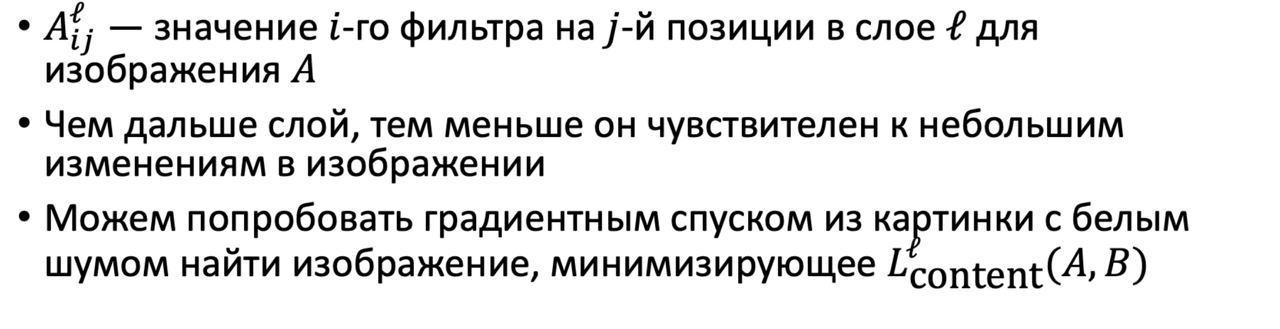
\includegraphics[width=0.7\linewidth]{1_contentnotation.jpg}
\caption{Нотация для первой компоненты Perceptual loss}
\label{fig:1_contentnotation}
\end{figure}
	
	Считаем для слоя l, он конкретный. Прогоняю картинку А в VGG беру слой нейросети l, там i канал (свертка i)  и смотрю ее значение на позиции j (позиция здесь просто индекс для всех возможных положений фильтра на картинке).
	
	Чем больше слой, тем более Loss будет отражать содержательные различия, а не какие-то непонятные мелкие признаки. 
	
	Возьмем значение этого лосса и будем ее минимизировать по B (пиксель), то есть мы будем менять изображение, чтобы добиться наименьшего лосса. 
	
	Лучше брать последние, если нам интересно содержимое. Картинка B меняется попиксельно. 
	
		\subsection{Style}
		
		
			\begin{equation}
	    L^{l}_{style}(A,B) = \sum_{i,j} (G^{l}_{i,j}(A) -G^{l}_{i,j}(B))^{2}
	    \label{eq:1_styletloss}
	\end{equation}
	
	Чтобы посчитать G для A, Мы берем два канала i и j, затем мы рассматриваем k-ю позицию фильтра  на указанных каналах. Перемножаем выходы с филтьтров и суммируем по всем k.
	
	\begin{equation}
	G^{l}_{i,j} (A) = \sum_{k} A^{l}_{i,k} \times  A^{l}_{j,k}
	   \label{eq:1_Gcompon}
	\end{equation}
	
	
	Что по сути происходит в \ref{eq:1_Gcompon}: эта штука показывает то, насколько перекликаются (насколько похожи) i и j канал с точки зрения выходов фильтра, проецируемеого на картинку А. 
	
	Обобщение всего лосса стилевого: он требует, чтобы корреляции каналов между собой (в нашем случае i,j) совпадали для картинки A и картинки B. 
	
	Затем предлагается взять таким образом полученные лосс для отдельных слоев l и просуммировать их с определенными весами. (В этом отличие от контентного лосса, там мы считали для одного слоя, а тут мы складываем по всем слоям). 
	
	
	
			\begin{equation}
	    L_{style}(A,B) = \sum^{L}_{l=0} w_l L^{l}_{style}(A,B)
	    \label{eq:1_styletloss}
	\end{equation}
	
	Как это понимать: 
	
	Допустим, что фильтр 1 детектирует человека (то есть там, тем больше выход, тем больше изображение похоже на человеческое), а фильтр 2 - синий цвет детектирует. Если стилевая картинка в синей гамме, то тогда корреляция между фильтрами будет высокая, поскольку тогда скалярное произведение будет большим. 
	
	Итоговый лосс будет выглядить следующим образом:
	
		\begin{figure}[H]
\centering
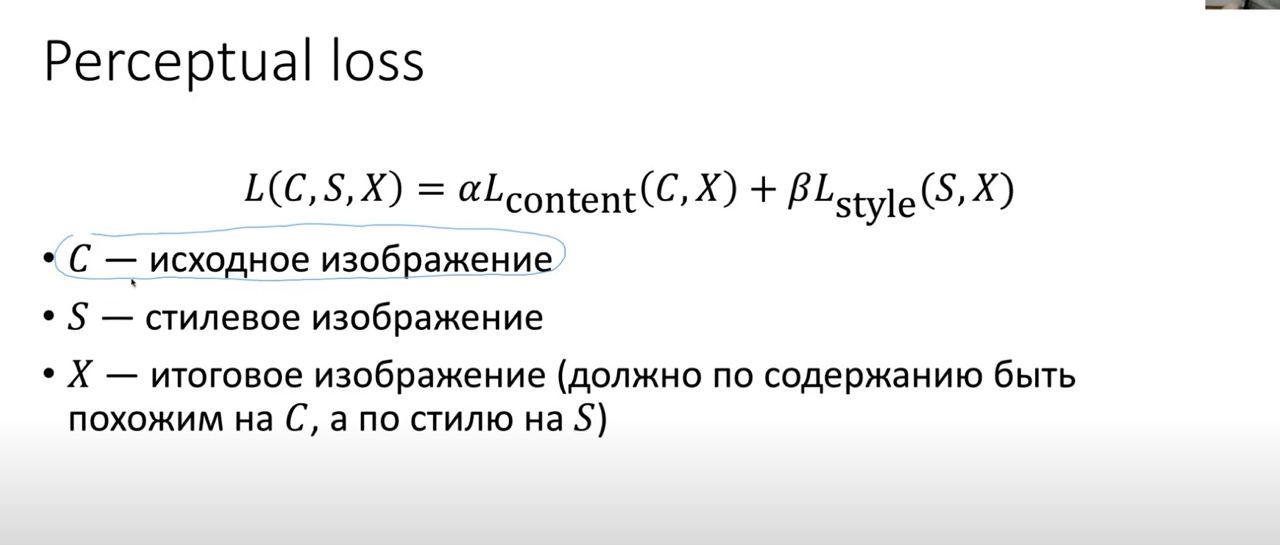
\includegraphics[width=0.7\linewidth]{1_finalloss.jpg}
\caption{Полный лосс}
\label{fig:1_finalloss}
\end{figure}


Нам дается "исходное" изображение, то есть которое мы пытаемся переделать (до этого это был белый шум). Хотим сделать похожим на S. X- результат. Как и с B, мы постоянно обновляем X для уменьшения лосса. $a$ и $\beta$ - гиперпараметры модели.  Минимизируем по X.  
	
